% Единый файл — все .tex файлы проекта объединены в один документ.
% Исходная структура: main.tex -> settings.tex, title.tex, task.tex,
%   task1.tex, task2.tex, task3.tex, conclusion.tex, appendix.tex

\documentclass[a4paper, final]{article}

% ============================================================
% settings.tex
% ============================================================
\usepackage[russian]{babel}
\usepackage{fontspec}
\setmainfont{Times New Roman}
\newfontfamily\cyrillicfonttt{Courier New}
\usepackage[14pt]{extsizes}
\usepackage[left=20mm, top=20mm, right=20mm, bottom=20mm, footskip=10mm]{geometry}
\usepackage{ragged2e}
\usepackage{indentfirst}
\usepackage{graphicx}
\usepackage{tikz}
\usepackage{caption}
\usepackage{xcolor}
\usepackage{subcaption}
\usepackage{listings}
\usetikzlibrary{arrows.meta}
\usepackage{nccmath}
\usepackage{soul}
\usepackage{algorithm}
\usepackage{algorithmic}
\usepackage{booktabs}
\usepackage{hyperref}
\usepackage{pdflscape}

\definecolor{link_color}{HTML}{0000EE}

\hypersetup{
    colorlinks=true,
    linkcolor=link_color,
    urlcolor=link_color,
    citecolor=link_color
}

\lstset{
    language=C++,
    basicstyle=\cyrillicfonttt\small,
    numbers=left,
    numberstyle=\tiny\color{gray},
    keywordstyle=\color{blue}\bfseries,
    commentstyle=\color{gray}\itshape,
    stringstyle=\color{red},
    frame=single,
    captionpos=b,
    breaklines=true,
    breakatwhitespace=false,
    showstringspaces=false,
    keepspaces=true,
    columns=flexible,
    fontadjust=true,
    basewidth={0.5em,0.45em},
    tabsize=4,
}

\begin{document}

% ============================================================
% title.tex
% ============================================================
{
\thispagestyle{empty}
\begin{center}
    \hfill \break
    \hfill \break
    МИНИСТЕРСТВО НАУКИ И ВЫСШЕГО ОБРАЗОВАНИЯ РОССИЙСКОЙ ФЕДЕРАЦИИ\\[5 pt]
    Федеральное государственное автономное образовательное учреждение высшего образования
    «Санкт-Петербургский политехнический университет Петра Великого»\\[10 pt]
    Институт компьютерных наук и кибербезопасности\\[5 pt]
    Направление: 02.03.01 Математика и компьютерные науки\\[30pt]


    {\large Отчет по дисциплине: «Вычислительная математика»}\\[30 pt]
    \LARGE\bf «Лабораторная работа №2».
\end{center}

\vspace{110 pt}

\begin{tabular*}{460pt}{@{\extracolsep{\fill}} l r}
     Студент,\tabularnewline группы 5130201/40003 \hspace{50pt}&  \line(1,0){100} \quad Адиатуллин Т. Р.\\
     & \\
     Руководитель,\tabularnewline Преподаватель & \line(1,0){121,5} \quad Пак В. Г.\\
     & \\
     & \\
     & \\
     & \guillemotleft \line(1,0){30} \guillemotright \line(1,0){100} \, 2026 \,г.

\end{tabular*} \\

\vfill

\begin{center}
    Санкт-Петербург, 2026
\end{center}
\newpage
}

\tableofcontents
\newpage

% ============================================================
% task.tex
% ============================================================
\section{Постановка задачи}

Для данной таблицы значений функции построить методом наименьших квадратов
линейную и квадратичную полиномиальные модели, вычислить наилучшие
среднеквадратические отклонения.

Функция $y = f(x)$ задана таблицей~\ref{tab:source}. Требуется построить её
аналитическое приближение. Для этого по данным таблицы находится функция
$y = g(x)$, аппроксимирующая исходную, т.е. удовлетворяющая условию
$g(x_i) \approx y_i$, $i = 1, \ldots, n$.

Аппроксимирующая функция строится из условия минимума среднеквадратического
отклонения:
\[
\delta_2(g) = \sqrt{\frac{1}{n}\sum_{i=1}^{n}(y_i - g(x_i))^2} \to \min.
\]

В данной работе аппроксимация проводится в классе алгебраических полиномов
степени $m$:
\[
P_m(x) = a_0 + a_1 x + \cdots + a_m x^m.
\]
Коэффициенты $a_0, a_1, \ldots, a_m$ находятся из нормальной системы МНК:
\[
\sum_{j=0}^{m} a_j \sum_{i=1}^{n} x_i^{j+k} = \sum_{i=1}^{n} y_i x_i^k,
\quad k = 0, \ldots, m.
\]

\begin{table}[h!]
\centering
\begin{tabular}{|c|c|c|c|c|c|c|c|c|c|c|}
\hline
$x_i$ & 0,1 & 0,2 & 0,3 & 0,4 & 0,5 & 0,6 & 0,7 & 0,8 & 0,9 & 1,0 \\
\hline
$y_i$ & 3,15 & 3,04 & 3,02 & 2,97 & 2,87 & 2,98 & 2,81 & 2,70 & 2,66 & 2,50 \\
\hline
\hline
$x_i$ & 1,1 & 1,2 & 1,3 & 1,4 & 1,5 & 1,6 & 1,7 & 1,8 & 1,9 & 2,0 \\
\hline
$y_i$ & 2,60 & 2,36 & 2,09 & 2,07 & 2,01 & 1,81 & 1,53 & 1,64 & 1,29 & 1,11 \\
\hline
\end{tabular}
\caption{Исходные данные функции $y = f(x)$.}
\label{tab:source}
\end{table}

\newpage

% ============================================================
% task1.tex
% ============================================================
\section{Линейная аппроксимация}

В этом разделе строится полином наилучшего среднеквадратического отклонения
степени $m = 1$, то есть линейная аппроксимация $P_1(x) = a_0 + a_1 x$.
Нормальная система МНК для её коэффициентов имеет вид:
\[
\begin{cases}
a_0 n + a_1 \displaystyle\sum_{i=1}^{n} x_i = \sum_{i=1}^{n} y_i, \\[6pt]
a_0 \displaystyle\sum_{i=1}^{n} x_i + a_1 \sum_{i=1}^{n} x_i^2 = \sum_{i=1}^{n} y_i x_i.
\end{cases}
\]

\subsection{Составление вспомогательной таблицы}

Для подстановки в нормальную систему вычислим необходимые суммы.
На листинге~\ref{lst:sums} приведён код, формирующий вспомогательную
таблицу~\ref{tab:aux}.

\begin{lstlisting}[caption={Вычисление вспомогательных сумм}, label=lst:sums]
import numpy as np

x = np.array([0.1,0.2,0.3,0.4,0.5,0.6,0.7,0.8,0.9,1.0,
              1.1,1.2,1.3,1.4,1.5,1.6,1.7,1.8,1.9,2.0])
y = np.array([3.15,3.04,3.02,2.97,2.87,2.98,2.81,2.70,2.66,2.50,
              2.60,2.36,2.09,2.07,2.01,1.81,1.53,1.64,1.29,1.11])

n    = len(x)
sx   = np.sum(x)        # sum xi
sx2  = np.sum(x**2)     # sum xi^2
sy   = np.sum(y)        # sum yi
sxy  = np.sum(x * y)    # sum xi*yi

print(f"n      = {n}")
print(f"sum x  = {sx:.4f}")
print(f"sum x2 = {sx2:.4f}")
print(f"sum y  = {sy:.4f}")
print(f"sum xy = {sxy:.4f}")
\end{lstlisting}

\begin{table}[h!]
\centering
\small
\begin{tabular}{|c|c|c|c|c|c|}
\hline
$i$ & $x_i$ & $y_i$ & $x_i^2$ & $x_i y_i$ \\
\hline
1  & 0,1 & 3,1500 & 0,0100 & 0,3150 \\
2  & 0,2 & 3,0400 & 0,0400 & 0,6080 \\
3  & 0,3 & 3,0200 & 0,0900 & 0,9060 \\
4  & 0,4 & 2,9700 & 0,1600 & 1,1880 \\
5  & 0,5 & 2,8700 & 0,2500 & 1,4350 \\
6  & 0,6 & 2,9800 & 0,3600 & 1,7880 \\
7  & 0,7 & 2,8100 & 0,4900 & 1,9670 \\
8  & 0,8 & 2,7000 & 0,6400 & 2,1600 \\
9  & 0,9 & 2,6600 & 0,8100 & 2,3940 \\
10 & 1,0 & 2,5000 & 1,0000 & 2,5000 \\
11 & 1,1 & 2,6000 & 1,2100 & 2,8600 \\
12 & 1,2 & 2,3600 & 1,4400 & 2,8320 \\
13 & 1,3 & 2,0900 & 1,6900 & 2,7170 \\
14 & 1,4 & 2,0700 & 1,9600 & 2,8980 \\
15 & 1,5 & 2,0100 & 2,2500 & 3,0150 \\
16 & 1,6 & 1,8100 & 2,5600 & 2,8960 \\
17 & 1,7 & 1,5300 & 2,8900 & 2,6010 \\
18 & 1,8 & 1,6400 & 3,2400 & 2,9520 \\
19 & 1,9 & 1,2900 & 3,6100 & 2,4510 \\
20 & 2,0 & 1,1100 & 4,0000 & 2,2200 \\
\hline
$\sum$ & 21,00 & 47,2100 & 28,7000 & 42,7030 \\
\hline
\end{tabular}
\caption{Вспомогательная таблица для нормальной системы МНК.}
\label{tab:aux}
\end{table}

\subsection{Решение нормальной системы}

Подставляя вычисленные суммы при $n = 20$, получаем нормальную систему для
линейной аппроксимации:
\[
\begin{cases}
20\,a_0 + 21{,}0000\,a_1 = 47{,}2100, \\
21{,}0000\,a_0 + 28{,}7000\,a_1 = 42{,}7030.
\end{cases}
\]

Решаем её с помощью кода, приведённого на листинге~\ref{lst:linear}.

\begin{lstlisting}[caption={Линейная аппроксимация МНК}, label=lst:linear]
import numpy as np

x = np.array([0.1,0.2,0.3,0.4,0.5,0.6,0.7,0.8,0.9,1.0,
              1.1,1.2,1.3,1.4,1.5,1.6,1.7,1.8,1.9,2.0])
y = np.array([3.15,3.04,3.02,2.97,2.87,2.98,2.81,2.70,2.66,2.50,
              2.60,2.36,2.09,2.07,2.01,1.81,1.53,1.64,1.29,1.11])

n   = len(x)
sx  = np.sum(x)
sx2 = np.sum(x**2)
sy  = np.sum(y)
sxy = np.sum(x * y)

# Нормальная система: A * a = b
A = np.array([[n,   sx ],
              [sx,  sx2]])
b = np.array([sy, sxy])

a0, a1 = np.linalg.solve(A, b)

# Аппроксимирующий полином и отклонение
P1      = a0 + a1 * x
delta1  = np.sqrt(np.sum((y - P1)**2) / n)

print(f"a0 = {a0:.4f},  a1 = {a1:.4f}")
print(f"P1(x) = {a0:.4f} + ({a1:.4f})*x")
print(f"delta2(P1) = {delta1:.4f}")
\end{lstlisting}

Решение нормальной системы даёт коэффициенты:
\[
a_0 = 3{,}4448, \quad a_1 = -1{,}0327.
\]
Таким образом, линейная аппроксимирующая функция имеет вид:
\[
P_1(x) = 3{,}4448 - 1{,}0327\,x.
\]

\subsection{Вычисление наилучшего среднеквадратического отклонения}

Наилучшее среднеквадратическое отклонение вычисляется по формуле:
\[
\delta_2(P_1) = \sqrt{\frac{1}{n}\sum_{i=1}^{n}(y_i - P_1(x_i))^2}.
\]
Подставляем сумму квадратов отклонений $\sum(y_i - P_1(x_i))^2 = 0{,}4286$:
\[
\delta_2(P_1) = \sqrt{\frac{1}{20} \cdot 0{,}4286} = 0{,}1464.
\]

\newpage

% ============================================================
% task2.tex
% ============================================================
\section{Квадратичная аппроксимация}

В этом разделе строится полином наилучшего среднеквадратического отклонения
степени $m = 2$, то есть квадратичная аппроксимация
$P_2(x) = a_0 + a_1 x + a_2 x^2$.
Нормальная система МНК для её коэффициентов:
\[
\begin{cases}
a_0 n + a_1 \displaystyle\sum x_i + a_2 \sum x_i^2
    = \sum y_i, \\[6pt]
a_0 \displaystyle\sum x_i + a_1 \sum x_i^2 + a_2 \sum x_i^3
    = \sum y_i x_i, \\[6pt]
a_0 \displaystyle\sum x_i^2 + a_1 \sum x_i^3 + a_2 \sum x_i^4
    = \sum y_i x_i^2.
\end{cases}
\]

\subsection{Дополнительные суммы}

Помимо сумм, найденных в разделе~2, потребуются ещё $\sum x_i^3$, $\sum x_i^4$ и
$\sum y_i x_i^2$. Они вычислены в таблице~\ref{tab:aux} и равны:
\[
\sum x_i^3 = 44{,}1000, \quad \sum x_i^4 = 72{,}2666, \quad
\sum y_i x_i^2 = 52{,}5719.
\]

\subsection{Решение нормальной системы}

Подставляя все суммы, нормальная система принимает вид:
\[
\begin{cases}
20\,a_0 + 21{,}0000\,a_1 + 28{,}7000\,a_2 = 47{,}2100, \\
21{,}0000\,a_0 + 28{,}7000\,a_1 + 44{,}1000\,a_2 = 42{,}7030, \\
28{,}7000\,a_0 + 44{,}1000\,a_1 + 72{,}2666\,a_2 = 52{,}5719.
\end{cases}
\]

На листинге~\ref{lst:quadratic} приведён код для решения этой системы.

\begin{lstlisting}[caption={Квадратичная аппроксимация МНК}, label=lst:quadratic]
import numpy as np

x = np.array([0.1,0.2,0.3,0.4,0.5,0.6,0.7,0.8,0.9,1.0,
              1.1,1.2,1.3,1.4,1.5,1.6,1.7,1.8,1.9,2.0])
y = np.array([3.15,3.04,3.02,2.97,2.87,2.98,2.81,2.70,2.66,2.50,
              2.60,2.36,2.09,2.07,2.01,1.81,1.53,1.64,1.29,1.11])

n    = len(x)
sx   = np.sum(x)
sx2  = np.sum(x**2)
sx3  = np.sum(x**3)
sx4  = np.sum(x**4)
sy   = np.sum(y)
sxy  = np.sum(x * y)
sx2y = np.sum(x**2 * y)

# Нормальная система: A * a = b
A = np.array([[n,   sx,  sx2],
              [sx,  sx2, sx3],
              [sx2, sx3, sx4]])
b = np.array([sy, sxy, sx2y])

a0, a1, a2 = np.linalg.solve(A, b)

# Аппроксимирующий полином и отклонение
P2     = a0 + a1 * x + a2 * x**2
delta2 = np.sqrt(np.sum((y - P2)**2) / n)

print(f"a0 = {a0:.4f},  a1 = {a1:.4f},  a2 = {a2:.4f}")
print(f"P2(x) = {a0:.4f} + ({a1:.4f})*x + ({a2:.4f})*x^2")
print(f"delta2(P2) = {delta2:.4f}")
\end{lstlisting}

Решение системы даёт коэффициенты:
\[
a_0 = 3{,}1147, \quad a_1 = -0{,}1323, \quad a_2 = -0{,}4287.
\]
Квадратичная аппроксимирующая функция:
\[
P_2(x) = 3{,}1147 - 0{,}1323\,x - 0{,}4287\,x^2.
\]

\subsection{Вычисление наилучшего среднеквадратического отклонения}

Наилучшее среднеквадратическое отклонение:
\[
\delta_2(P_2) = \sqrt{\frac{1}{n}\sum_{i=1}^{n}(y_i - P_2(x_i))^2}.
\]
Сумма квадратов отклонений $\sum(y_i - P_2(x_i))^2 = 0{,}1059$, поэтому:
\[
\delta_2(P_2) = \sqrt{\frac{1}{20} \cdot 0{,}1059} = 0{,}0728.
\]

Таблица~\ref{tab:dev} содержит значения $P_1(x_i)$, $P_2(x_i)$ и квадраты
отклонений для каждого узла.

\begin{table}[h!]
\centering
\small
\begin{tabular}{|c|c|c|c|c|c|c|}
\hline
$i$ & $x_i$ & $y_i$ & $P_1(x_i)$ & $(y_i - P_1)^2$ & $P_2(x_i)$ & $(y_i - P_2)^2$ \\
\hline
1  & 0,1 & 3,1500 & 3,3416 & 0,0367 & 3,0972 & 0,0028 \\
2  & 0,2 & 3,0400 & 3,2383 & 0,0393 & 3,0711 & 0,0010 \\
3  & 0,3 & 3,0200 & 3,1350 & 0,0132 & 3,0364 & 0,0003 \\
4  & 0,4 & 2,9700 & 3,0318 & 0,0038 & 2,9932 & 0,0005 \\
5  & 0,5 & 2,8700 & 2,9285 & 0,0034 & 2,9414 & 0,0051 \\
6  & 0,6 & 2,9800 & 2,8252 & 0,0240 & 2,8810 & 0,0098 \\
7  & 0,7 & 2,8100 & 2,7219 & 0,0078 & 2,8120 & 0,0000 \\
8  & 0,8 & 2,7000 & 2,6187 & 0,0066 & 2,7344 & 0,0012 \\
9  & 0,9 & 2,6600 & 2,5154 & 0,0209 & 2,6483 & 0,0001 \\
10 & 1,0 & 2,5000 & 2,4121 & 0,0077 & 2,5536 & 0,0029 \\
11 & 1,1 & 2,6000 & 2,3089 & 0,0848 & 2,4503 & 0,0224 \\
12 & 1,2 & 2,3600 & 2,2056 & 0,0238 & 2,3385 & 0,0005 \\
13 & 1,3 & 2,0900 & 2,1023 & 0,0002 & 2,2181 & 0,0164 \\
14 & 1,4 & 2,0700 & 1,9991 & 0,0050 & 2,0891 & 0,0004 \\
15 & 1,5 & 2,0100 & 1,8958 & 0,0130 & 1,9515 & 0,0034 \\
16 & 1,6 & 1,8100 & 1,7925 & 0,0003 & 1,8054 & 0,0000 \\
17 & 1,7 & 1,5300 & 1,6892 & 0,0254 & 1,6507 & 0,0146 \\
18 & 1,8 & 1,6400 & 1,5860 & 0,0029 & 1,4874 & 0,0233 \\
19 & 1,9 & 1,2900 & 1,4827 & 0,0371 & 1,3155 & 0,0006 \\
20 & 2,0 & 1,1100 & 1,3794 & 0,0726 & 1,1350 & 0,0006 \\
\hline
$\sum$ & & & & 0,4286 & & 0,1059 \\
\hline
\end{tabular}
\caption{Значения аппроксимирующих полиномов и квадраты отклонений.}
\label{tab:dev}
\end{table}

\newpage

% ============================================================
% task3.tex
% ============================================================
\section{Графики и сравнение аппроксимаций}

Для наглядного сравнения исходных данных с построенными моделями построим графики.
На листинге~\ref{lst:plot} приведён соответствующий код.

\begin{lstlisting}[caption={Построение графиков аппроксимаций}, label=lst:plot]
import numpy as np
import matplotlib.pyplot as plt

x = np.array([0.1,0.2,0.3,0.4,0.5,0.6,0.7,0.8,0.9,1.0,
              1.1,1.2,1.3,1.4,1.5,1.6,1.7,1.8,1.9,2.0])
y = np.array([3.15,3.04,3.02,2.97,2.87,2.98,2.81,2.70,2.66,2.50,
              2.60,2.36,2.09,2.07,2.01,1.81,1.53,1.64,1.29,1.11])

# Коэффициенты (найденные ранее)
a0_1, a1_1 = 3.4448, -1.0327
a0_2, a1_2, a2_2 = 3.1147, -0.1323, -0.4287

x_fine = np.linspace(0.1, 2.0, 300)
P1_fine = a0_1 + a1_1 * x_fine
P2_fine = a0_2 + a1_2 * x_fine + a2_2 * x_fine**2

plt.figure(figsize=(8, 5))
plt.scatter(x, y, color='blue', zorder=5, label='Исходные данные')
plt.plot(x_fine, P1_fine, color='black', linewidth=1.5, label=r'$P_1(x)$ — линейная')
plt.plot(x_fine, P2_fine, color='red',   linewidth=1.5, label=r'$P_2(x)$ — квадратичная')
plt.xlabel('x')
plt.ylabel('y')
plt.title('Аппроксимация методом наименьших квадратов')
plt.legend()
plt.grid(True)
plt.tight_layout()
plt.savefig('approximation.png', dpi=150)
plt.show()
\end{lstlisting}

На рисунке~\ref{fig:approx} изображены исходные данные и обе аппроксимирующие
кривые. Видно, что квадратичная модель $P_2(x)$ значительно точнее следует за
табличными данными по сравнению с линейной $P_1(x)$.

\begin{figure}[h!]
\centering
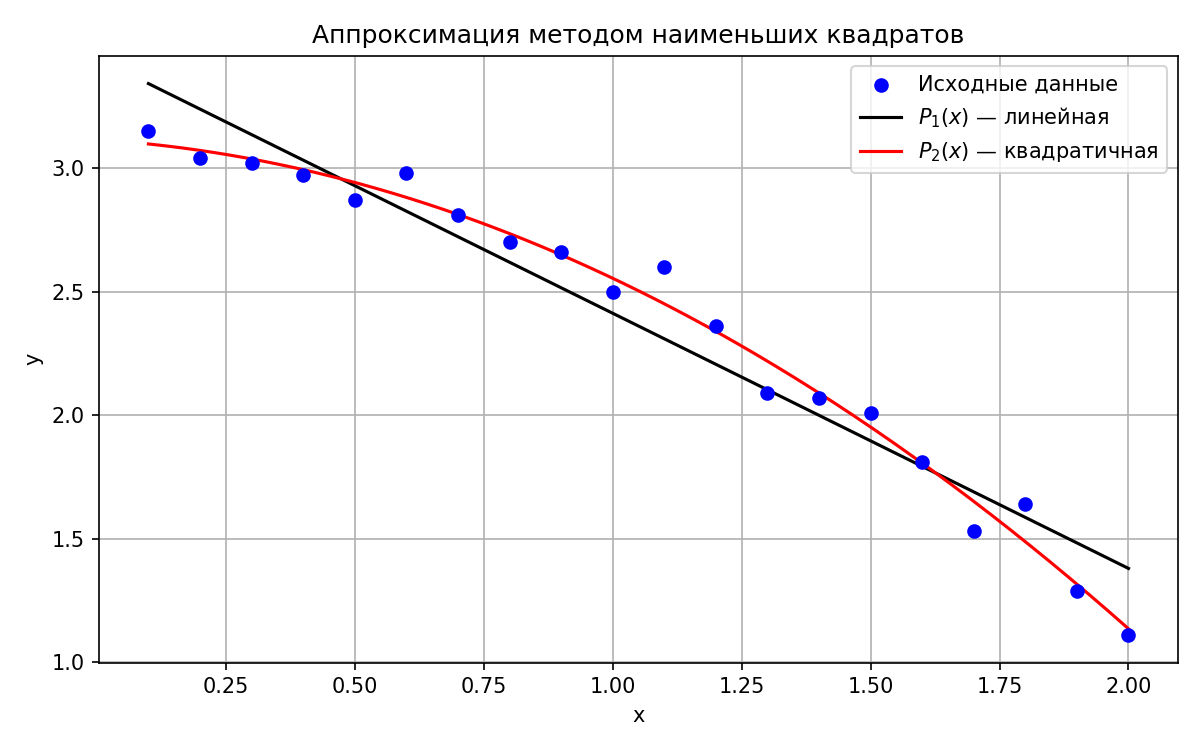
\includegraphics[width=0.85\textwidth]{approximation.png}
\caption{Графики исходных данных и аппроксимирующих полиномов.}
\label{fig:approx}
\end{figure}

\newpage

% ============================================================
% conclusion.tex
% ============================================================
\section*{Заключение}
\addcontentsline{toc}{section}{Заключение}

В ходе выполнения лабораторной работы была изучена полиномиальная аппроксимация
методом наименьших квадратов. По таблице из $n = 20$ узлов были построены два
аппроксимирующих полинома.

Для линейной аппроксимации $P_1(x) = a_0 + a_1 x$ нормальная система МНК
была составлена и решена, в результате чего получены коэффициенты
$a_0 = 3{,}4448$ и $a_1 = -1{,}0327$:
\[
P_1(x) = 3{,}4448 - 1{,}0327\,x.
\]
Наилучшее среднеквадратическое отклонение составило $\delta_2(P_1) = 0{,}1464$.

Для квадратичной аппроксимации $P_2(x) = a_0 + a_1 x + a_2 x^2$ получены
коэффициенты $a_0 = 3{,}1147$, $a_1 = -0{,}1323$, $a_2 = -0{,}4287$:
\[
P_2(x) = 3{,}1147 - 0{,}1323\,x - 0{,}4287\,x^2.
\]
Наилучшее среднеквадратическое отклонение составило $\delta_2(P_2) = 0{,}0728$.

Квадратичная модель вдвое точнее линейной: $\delta_2(P_2) < \delta_2(P_1)$.
Это закономерно, поскольку полином более высокой степени обладает большей
гибкостью при подгонке к данным. Все вычисления выполнены программно на языке
Python с использованием библиотеки NumPy.

\end{document}
